


\begin{comment}
The key of the conversion is to incrementally compute the origin problem and the difference value $\Delta X^k$ of each recursion can be iteratively computed i.e.
 
\begin{equation}
\label{eq:con}
\begin{aligned}
X^{k+1}=&X^k+\Delta X^k\\
\Delta X^{k}=&G' \circ F' (\Delta X^{k-1}).
\end{aligned}
\end{equation}
if aggregate function $G'$ satisfied the \textbf{accumulative} condition, the first line of equation \ref{eq:con} can be rewrite as $X^{k+1}=G'(X^0\cup \Delta X^0\cup \Delta X^1 \ldots \Delta X^k)$.%Note that $G'$ is not necessarily the origin $G$,usually it depends on specific questions.
This is the basic formula of accumulative recursive aggregation which has the same result with normal recursive aggregation .Algorithm can be correctly asynchronized if the \textbf{order-independent} conditions satisfied. Though the basic idea has been proposed,there are still two key problems to be solved. First, how to determine the new aggregation function $G'$. Second,How to determine the incremental value $\Delta X^k$ from $X^k$ and $X^{k+1}$.
Third, how to initialize the incremental value $\Delta X^0$.


Since the new aggregation $G'$ express the relationship between $\Delta X^k$ and $\Delta X^{k-1}$. So the relation can be obtained by evaluate the incremental value between two adjacent recursion. First define the calculation of incremental value as $\Delta X^{k}=diff(X^{k+1},X^{k})$ in which $diff( \cdot , \cdot )$ is a inverse transformation of $G'$, i.e., $X^{k+1}=G'(X^k \cup diff(X^{k+1},X^{k}))$. Then we can try to find a $G'$ satisfied that $diff(G\circ F(X^{k+1}),G \circ F(X^{k})) = G'\circ F(diff(X^{k+1},X^{k}))$. If $G'$ exists and satisfied the community condition, the original algorithm  can be converted. Otherwise, the algorithm can't be converted. 

Usually it is hard to find suitable $G'()$ for an arbitrary algorithm, because it is hard to determine $G'()$ and its inverse transformation $diff()$ at the same time. And even for some aggregate functions there is no inverse transformation to determine the relation between $\Delta X^k$ and $X^k$,$X^{k-1}$.e.q., MIN and MAX. So In this section we only concern about the algorithm with 'SUM' aggregate operations and its variety. Because a large amount of algorithm can be expressed with SUM  operations in their aggregate function. And a lot of them has the ability to accumulatively computing. {\color{red} I want to express that sum is used widely in many algorithm, and even though we only learn the Sum operation, it is still meaningful} For SUM operation and its variety, $diff(X^{k+1},X^{k})$ is the difference between each two adjacent recursion, i.e., subtract each element of the vector correspondingly.

Since we define $\Delta X^k=diff(X^{k+1},X^{k})$,and we have $X^{k+1}=G'(X^0\cup \Delta X^0 \cup G'\circ F'(\Delta X^0)\cup \ldots G' \circ F^n(\Delta X^0))$. To determine $\Delta X^0$,  We can perform normal recursive aggregation for one time and obtain $X^1$. Then $\Delta X^0$ is initialized as $diff(X^1,X^0)$ and $X^0$ is still $X^0$. Then the algorithm can be accumulatively executed.

%\cite{maiter}.
In original PageRank, $R^k=(1-b)AR^{k-1}+b$, where $A$ is a matrix that represents the graph structure. $F$ operation is sending rank value $R_i$ to their outgoing neighbor, corresponding to the multiplication by subscript of transform matrix $A$,$G$ operation is the 'SUM' of intermediate result by the row number of $A$ with constant vector $b$ added. following the define of $diff(\cdot,\cdot)$,
\begin{equation}
\Delta R^k=(1-b)A\Delta R^{k-1}\notag
\end{equation}
So we can obtain that $X^k=X^0+\Delta X^0+(1-b)A\Delta X^0+\ldots+((1-b)A)^{k-1}\Delta X^0$
where $\Delta X^0$ is initialized as $X^1-X^0$. The $F$ operation is matrix multiplication without summing up,and $G$ operation is the 'SUM' of the intermediate result.
Furthermore, $g'$ operation is accumulative,the $f()$ operation and $g'()$ operation in PageRank is order independent($F$,$G'$ is the same), e.q., $\sum_{n}{0.8*x_i/d}=0.8/d*\sum_{n}{x_i}$ which makes it suitable for asynchronous aggregation. There also exist other convertible algorithms, such as Program(8,11,12,
13) in Appendix Sec. \ref{sec:app:example}. 


Next, we formally provide the convertibility conditions as follows.

\begin{theorem}
	\label{th:convert}
	(\textbf{Convertibility}) A recursive program can be converted to an accumulated recursive program for asynchronous aggregation, as long as an aggregate operation $G'()$ with the \textbf{accumulative} and \textbf{commutative} properties can be found with the following conditions:\\
	\begin{itemize}
		\item \textbf{convertible}: $G\circ F(X^{k+1})=G'(X^k\cup G'\circ F(\Delta X^k))$
\item \textbf{eliminable}: $\vert\vert lim_{n\rightarrow\infty}(G'\circ F)^n(x)\vert\vert=\textbf{0}$,
	\end{itemize}
	 The $G'()$ operation is the aggregate operation in the new accumulated recursive program.
\end{theorem}

The formal proof can be found in Appendix Sec. \ref{sec:app:proof:convert}. 
Note that, it is not realistic to perform recursion infinite times. In practice, we will stop the recursion as long as the incremental value $(G'\circ F)^n(x)$ is ``small'' enough.

\end{comment}




\section{Automatic Asynchronization}
\label{sec:async:autoasync}

\subsection{Converting Nonmonotonic program to Semi-Naive Evaluation}
\label{sec:async:convert}

As discussed above, the primary requirement for asynchronous aggregation is that the recursive program is an accumulated recursive program. %{\color{red} in other words,  The progranm can be semi-naive evaluated}.
However, a large number of recursive algorithms do not satisfy the accumulable requirement as definition \ref{def:araggre}. Especially the monotonic requirement of non-aggregate operations $F$ and the ideopotent property also restrict the application os asynchronous processing . However some algorithms that doesn't satisfied the monotonic condition still have the possibility to convert to accumulative recursive aggregation .So in this section, we will introduced a convert technology to guide the trasnformation.


\textbf{Example 2: What is the cost of each part}
\small
\begin{lstlisting}
r1. cost(Part,$\mathcal{C}$) $\leftarrow$ basic(Part,cost).
r2. cost(Part,sum[$\mathcal{C}$]) $\leftarrow$ assb(Part,Sub,$n$),
cost(Sub,$c$), $\mathcal{C}=c*n$;
basic(Part,$\mathcal{C}$).
\end{lstlisting}
\normalsize



\textbf{Example 3: PageRank}
\small
\begin{lstlisting}
r1. degree(X,count[Y])$\leftarrow$ edge(X,Y).
r2. rank(X,$r$) $\leftarrow$ node(X),$r=1$.
r3. rank(Y,sum[$r$]) $\leftarrow$  Node(Y), r=0.15;
rank(X,$r1$), edge(X,Y),
degree(X,$d$), $r=0.85\cdot r1/d$.
\end{lstlisting}
\normalsize

% The PageRank computation is another typical recursive program for ranking the nodes in a graph. The ranking score is initialized as $r_i^0=1/|V|$ for each node $i$ where $|V|$ is the total number of nodes. The $f()$ operation for node $i$ takes a tuple $\langle i,r_i^k\rangle$ as input where $r_i^k$ is the ranking score in the $k$th recursion, computes $f(r_i^k)=0.85*r_i^k/d_i=tr_j^{k+1}$ for any outgoing neighbors $j$ and $0.15$ for itself(where 0.85 is the constant damping factor and $d_i$ is the out-degree of node $i$), and outputs the tuples set $\{\langle j,tr_j^{k+1}\rangle\}$. The aggregate operation $g()$ with respect to each node $j$ takes the input tuples $\{\langle j,tr_j^{k+1}\rangle\}$ and constant  $0.15$, performs the SUM aggregation $g(\{\{tr_j^{k+1}\},0.15\})=\sum_j{tr_j^{k+1}}+0.15=r_j^{k+1}$ and outputs $\langle j,r_j^{k+1}\rangle$. It terminates when the difference between two continuous recursions' ranking scores is small enough.

With regard to Cost algorithm, the monotonic condition (i.e., $X\in F(X)$) is not satisfied. After applying the $F(X^{k})$ operation, it produces a new set of kv-pairs representing the outgoing messages to neighbors  without preserving the old kv-pairs. {\color{green}that represent the ranking scores of vertices} (new Total cost  will be calculated based on the cost of sub part and the basic cost of itself ). In other words, the aggregation result $X^{k}$ is replaced by $F(X^{k})$ but not contained in $F(X^{k})$.

Fortunately, a number of recursive algorithms that are not originally accumulable can be equivalently converted into accumulated recursive programs by changing the original recursive form, as long as two conditions are satisfied.


{\color{red}

The first requirement is that{\color{blue} the aggregate operation is $\$sum$ } the results can be incrementally computed. then we define $\Delta^{k}$ as the increment between each two recursion i.e., $\Delta^{k}=X^k-X^{k-1}$. Then the program can be evaluated with $X^k=G^+(\cup_{i=1}^{k}\Delta^i\cup X^0)$.
% $ G^+\circ F(X^{k})=G^+(X^{k}\cup F'(\Delta^{k-1}))$.
%In which $G^+$ is the aggregate function, and $F'$ is an new non-aggregate operation for $\Delta$ computing.

%and denote
%$\Delta X^{k}=G^+\circ F(X^k)-X^{k}$ i.e., $G^+\circ F(X^{k})=G^+(X^{k}\cup G^+\circ F(X^k)-X^{k})$.
Further, as defined in Equation \ref{eq:accumasync}, the increment $\Delta^{k}$ should be computed based on $\Delta^{k-1}$ using the same aggregate functions $G^+$ and new non-aggregate operation $F'$, i.e., $\Delta^{k}=G^+\circ F'(\Delta X^{k-1})$.
Then the Original form $(G^+\circ F)^k(X^0)$ can be converted to
\begin{equation}
\label{eq:convertform}
\begin{aligned}
&(G^+\circ F)^k(X^0)
=G^+( \cup_{i=0}^{k-1}{(G\circ F)^i(\Delta^{1})\cup X^0})
%=&G^+(X^0\cup\Delta^0\cup G^+\circ F'(\Delta^0)\ldots \cup (G^+\circ F')^{k-1}(\Delta^0))
\end{aligned}
\end{equation}
Take COST algorithm as an example, the original COST program using $\$sum$ as aggregate operations. But the algorithm can be incrementally evaluated, the F operations contains two part 1) send self-total-cost times number to the higher level part, 2)get the basic cost of ites self.  Then the new $F'$ operation is the previous $F$ with second operation removed. The new program start from the basic cost of each part, and the cost of each sub part can be incrementally evaluated, e.g., Only the difference of cost is accumulated. The program terminated when there is no new difference produced.

While the question rised that how to determine a new non-aggregate operation $F'$? Since
%$G^+\circ F(X^{k})=G^+(X^{k}\cup\Delta^{k})$,
\begin{equation}
\label{eq:inferr}
\begin{aligned}
\Delta^k&=X^k-X^{k-1}\\
G^+(\Delta^{k})&=G^+(X^k-X^{k-1})\\
G^+(\Delta^{k})&=G^+(G^+\circ F(X^{k-1})-G^+\circ F(X^{k-2}))\\
\Delta^{k}&=G^+(F(X^{k-1})-F(X^{k-2}))\notag
\end{aligned}
\end{equation}
Then
\begin{equation}
\label{eq:findf}
\begin{aligned}
&G^+\circ F'(\Delta^{k})=G^+(F(X^{k})-F(X^{k-1})).
\end{aligned}
\end{equation}
}

{\color{green}
The first requirement is that the aggregation is SUM. Then the increment of aggregation results can be computed as $\Delta X^k=X^{k+1}-X^k$. Note that, since $X$ is a kv-pairs set with unique keys, the `$+$'/`$-$' operation over two kv-pairs set denotes pair-wise value summation/subtraction indexed by key. As defined in Equation \ref{eq:accumasync}, the increment $\Delta X^{k+1}$ should be computed based on $\Delta X^k$, i.e., $\Delta X^{k+1}=G^{+}\circ F'(\Delta X^k)$ where $G^{+}$ represents the group-by SUM aggregation referring to our first SUM operation requirement, and $F'$ is a new non-aggregate function. To find a feasible $F'$, since $\Delta X^{k+1}=G^{+}\circ F'(\Delta X^k)$, we have $X^{k+2}-X^{k+1}=G^{+}\circ F'(X^{k+1}-X^k)$. Further, we have
}

This is the second requirement that help us find a feasible non-aggregate operation $F'$ according to the current $F$ function. However is is still hard to get the non-aggregate formula directly through the equation \ref{}. Because of the coupling of multiple conditions. So we introduce an automatic determine technology by leveraging Z3 SMT solver.
{\color{green} There is one more question we should answer before proposing the new accumulated recursive program. How to initialize $\Delta X^0$? To initialize $\Delta X^0$,  We can perform the normal recursive program for one iteration to obtain $X^1$, and set $\Delta X^0=X^1-X^0$ where $X^0$ is the initial value in original recursive program.

Given the new accumulated recursive program with $G^+$ and $F'$, we aim to find the conditions that guarantee the convergence and correctness. With an initial $X^0$, the final result of original recursive program is $(G^{+}\circ F)^n(X^0)$, while the final result of the new accumulated recursive program is $X^0+\Delta X^0+G^+\circ F'(\Delta X^0)+\ldots+(G^+\circ F')^n(\Delta X^0)$. By applying equation \ref{eq:findf} to $(G^{+}\circ F)^n(X^0)$, we have $X^0+\Delta X^0+\ldots+(G^+\circ F')^n(\Delta X^0)+(G^+\circ F')^{n+1}(\Delta X^0)$. When $(G^+\circ F')^{n+1}(\Delta X^0)$ is approaching to \textbf{0} (i.e., the values of all kv-pairs are approaching to 0), the result of the new accumulated recursive program is approaching to that of the original program.
}

Therefore, we have the following definition to guide convertion.
\begin{definition}
\label{th:convert}
A convertiable recursive program can be converted to an accumulated recursive program as equation \ref{eq:convertform} and return the same results after $n$ iterations with naive-evaluation, as long as the following conditions are satisfied:
\begin{itemize}
	\item The aggregate operation $G^+$ is $\$sum$ operations.{\color{blue} this  might has a high level statement please keep this mark here or totally removed this part}
	
	\item The original program can be incrementaly evaluated with $X^{k}=G^+(X^{k-1}\cup \Delta^{k-1})$
	\item There exists an non-aggregate operation $F'$ satisfitd that $\Delta^{k}=G^+\circ F'(\Delta X^{k-1})$
	%\item The increment can be iteratively evaluated with non-aggregate operation $F'$ i.e.,   $\Delta^{k+1}=G^+\circ F'(\Delta X^{k})$
	%\item There exists an non-aggregate operation $F'$ satisfitd that $G^+\circ (F(X^{k-1})-F(X^{k-2}))=G^+\circ F'(\Delta^{k-2}).$
	%		\item The initial $\Delta^0$ is defined as $X^1-X^{0}$ with naive evaluation result.
	
	
	%		\item With the initialization $\Delta X^0=X^1-X^0$, we have $(G^+\circ F')^{n+1}(\Delta X^0)=\textbf{0}$.
\end{itemize}
\end{definition}
{\color{green}
Note that, the last condition can be relaxed with condition $lim_{n\rightarrow\infty}(G\circ F')^n(\Delta X^0)=0$ to obtain an approximate result.
}


In System implementation, the initial value of $\Delta^1$ could be init with $X^1-X^0$ by performing naive-evaluation for one time.

PageRank is another recursive program that can be converted to the accumulated recursive program. The $G$ operation is $\$sum$. The new $F'$ operation is $f(r_i^k)=0.85*r_i^k/d_i$ without adding the constant 0.15 to itself. Further, after an infinite number of iterations we have $lim_{n\rightarrow\infty}(G\circ F')^n(\Delta X^0)=0$ due to the contraction property. There also exist some other convertible algorithms, such as COST algorithm, Belief Propagation, Simrank and Jacobi method. The datalog programs are detailed in technical report\cite{fullversion}.





\subsection{Automatation}
\begin{figure}[!t]
	\centering
	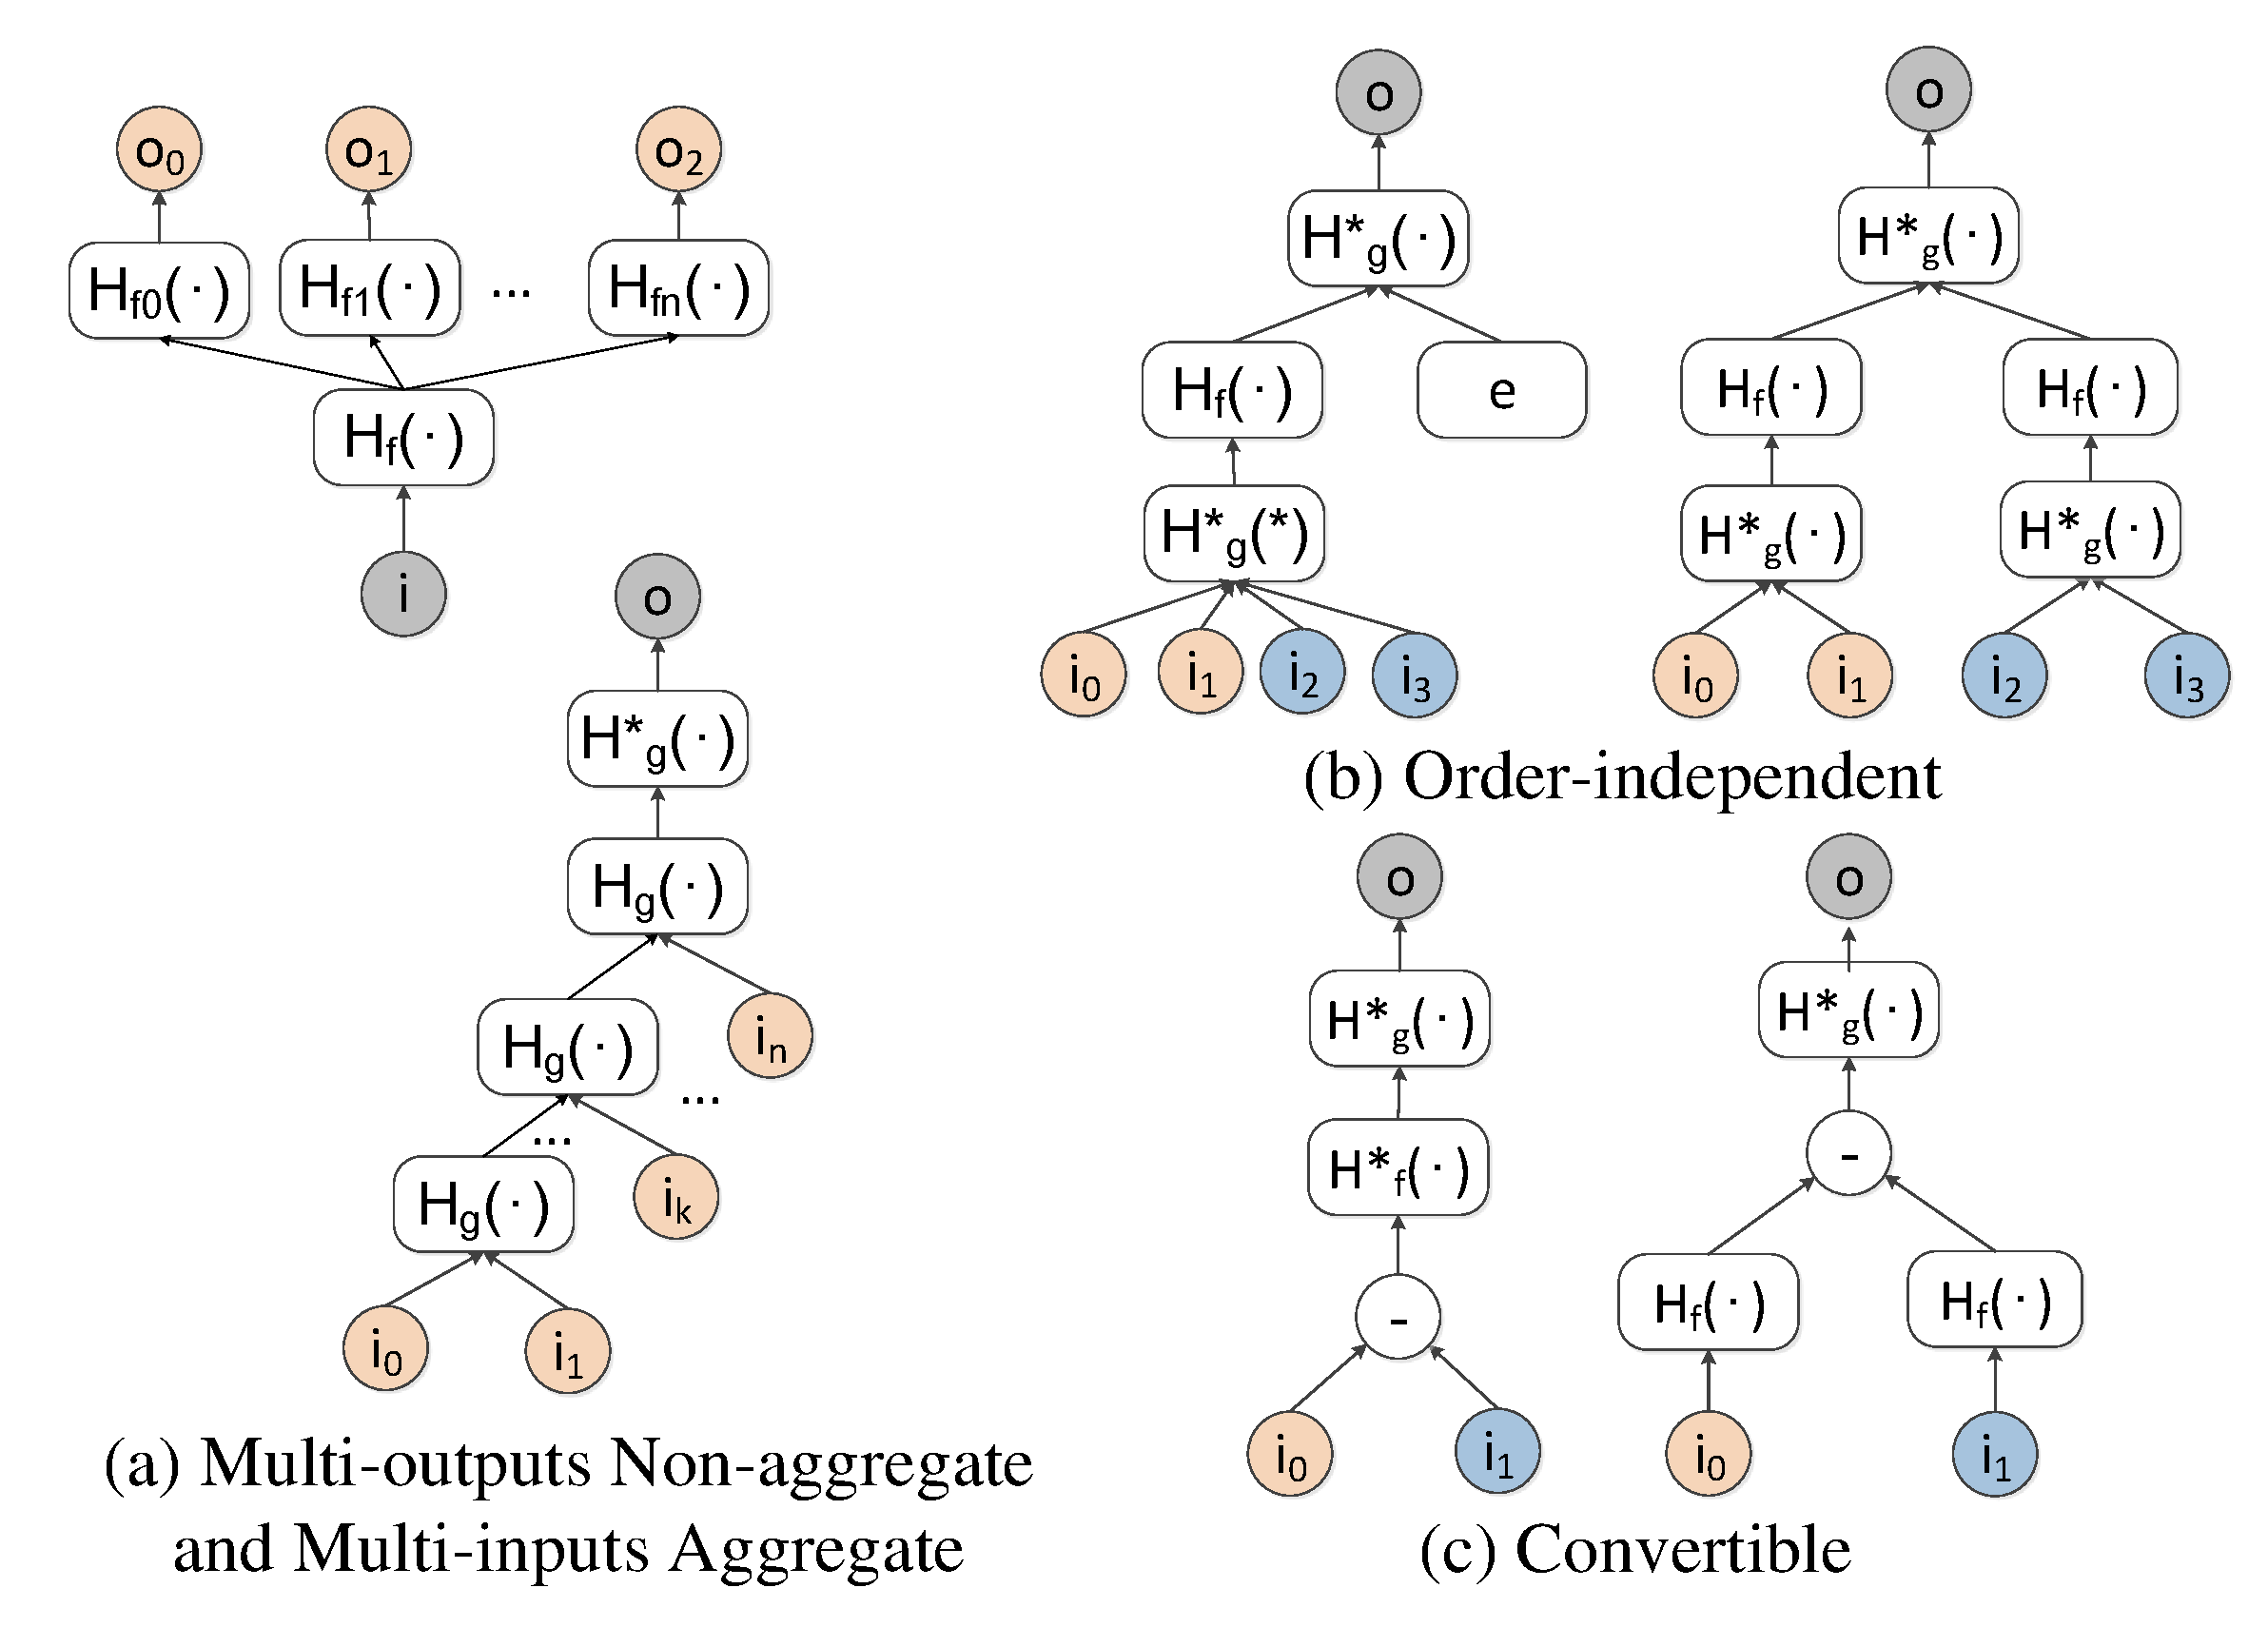
\includegraphics[width=3.2in]{figuration/automodel.pdf}
	\vspace{-0.1in}
	\caption{Expression Construction}
	\label{fig:automodel}
	\vspace{-0.1in}
\end{figure}
Though the conditions for asynchronous aggregation have been identified, it is still hard for a non-expert programmer to verify these complex conditions manually. And it is also hard to find a new function $F'()$ for converting a normal recursive program into an accumulated recursive program.
 To alleviate the burden of programmers, an automatic asynchronization scheme is desired. In this section, we discuss how to automatically verify these conditions given the $g()$ and $f()$ operations. To simplify the analysis, we use key-specific operations $g$ and $f$ to describe the automation process instead of using the set oriented operations $G$ and $F$.
 
\Paragraph{Condition Checker}
The monotonic conditions can be easily checked by the struct of Datalog program. if the Table to be aggrgate is apperaing on both side of the recursive rule with same key, then the monotonic property is satisfied. The other condition verification problems can be thought of as a form of the constraint satisfaction problem, which can be analyzed with the help of \emph{satisfiability modulo theories} (SMT) \cite{53e486195688442995f82bfe28c55731}. The satisfiability of these conditions can then be checked by an SMT solver, such as Z3 \cite{DeMoura:2008:ZES:1792734.1792766}. Next, we show how to reduce these condition verification problems into SMT satisfiability solving problems.

The nonaggregate operation is constract with relation and output expression, and there might be several output expression in one rules e.g., the example 2, in \texttt{r2.}, the $f$ is divided into two parts:
\begin{lstlisting}
1. assb(Part,Sub,$n$), cost(Sub,$c$), $\mathcal{C}=c*n$;
2. basic(Part,$\mathcal{C}$).
\end{lstlisting}
Sothe output expression of non aggregate operation is also consist of the part, $\mathcal{C}=c*n$ and  $\mathcal{C}$. The property of $f$ is only depend on the form of unique expression .


In order to translate $g$ and $f$ into a formula for being verified by an SMT solver, we implement a serie of unary function $H_{fi}(\bullet)$  to represent the $i$th output expression of $f$, and Binary function $H_g(\bullet,\bullet)$ to represent aggregate operation $g$. If the accumulative property is satisfied
We can further define $H^n_g(\bullet)$ for $n$ inputs aggregation by recursively apply $H_g(\bullet,\bullet)$.
Then all the condition check problem can be construct with these two function.

\textcolor{blue}{ Given a function $H=\{f(x_1),\ldots,f(x_m)\}$ or $H=\{g(x_1),...g(x_n)\}$, we are interested in a formula for $H$ of the form $\phi_H^{o_1,\ldots,o_m}$, where $o_1,\ldots,o_m$ are output variables \cite{Liu:2014:ADP:2670979.2670980}. Intuitively, the formula $\phi$ is ``correct'' if an assignment to $\{x_1,\ldots,x_n,o_1,\ldots,o_m\}$ makes $\phi$ be true if and only evaluating $H(x_1,\ldots,x_n)$ returns $o_1,\ldots,o_m$. Then the satisfiability of $\phi$ exactly implies that the function will compute the same output. Based on this formula, we present the formulas for different conditions in the following.
}
For the accumulative, idempotent, and commutative conditions in definition \ref{th:monotone} and the order independent condition in definition\ref{th:async}, the condition verification problems can be reduced to SMT satisfiability problems via the following equation.

\begin{definition}
	\label{coro:auto:1}
	(\textbf{Accumulative, Commutative, Idempotent and Order Independent})
	\textcolor{blue}{$\forall_{i=1\to m} \{x_{1i},x_{2i},x_{3i}\}$, the condition 1 or 2 or 3 is true if and only if $\phi_{H_l}^{o1,\ldots,o_m}\wedge \phi_{H_r}^{o_1',\ldots,o_m'}\wedge (\vee_{i=1}^m{o_i\neq o_i'})$ is not satisfiable, where}
	
	Denote $H_f(*)$ as set of the output expression, e.g., $H_f(*)=\{H_{f0}(*),H_{f1}(*)\ldots H_{fn}(*)\}$. And denote $e$ as the identical element of binary function $G$,
	The condition is satisfied  if $H_l=H_r$. 
	\begin{itemize}
		\item condition 1: accumulative, $H_l=H_g(x_1,H_g(x_2,x_3))$ and $H_r=H_g(H_g(x_1,x_2),x_3)$;
		\item condition 2: commutative, $H_l=H_g(x_1,x_2)$ and $H_r=H_g(x_2,x_1)$;
		\item condition 3: idempotent, $H_l=H_g(x_1,x_2)$ and $H_r=H_g(x_2,x_1)$;
		\item condition 4: order independent, \\		
		$H_l=H^*_g(H_f(H^*_g(x_1,x_2,x_3,x_4)),e)$\\		
		 and  $H_r=H^*_g(H_f(H^*_g(x_1,x_2)),H_f(H^*_g(x_3,x_4)))$;
	\end{itemize}
\end{definition}
{\color{green}
Note that, SMT cannot judge ``whether a formula $H$ is always true?'' but only answers ``whether a formula $H$ is satisfiable?''. A formula $H$ is \emph{satisfiable} if there is some assignment of appropriate values to its uninterpreted function and constant symbols under which $H$ evaluates to true. Thus, to verify a condition (that should be always true), we convert the ``$H$ is always true'' problem to the ``not $H$ is not satisfiable'' problem. If $H$ is always true, then ``not $H$'' is always false, and then ``not $H$'' will not have any satisfying assignment
}

\Paragraph{Founding New Non-aggregate Operation}
Furthermore, SMT solver Z3 can be used to find a qualified $f'$ function for auto conversion. Following Corollary \ref{coro:auto:1}, we first use Z3 to check the satisfiability. 
If the formula is satisifiable system will directly obtain $f'$ by remove $X$ from $F$.
If the formula is not satisfiable, system will try to find a new $f'$ based on the original non-aggregate operation $f$ by the method proposed in equation \ref{eq:findf}. As discuessed above the operation $H_f$ might contains multi expression. So we first remove the constant expression in $f$ to obtain the candidate $H^*_f$ and then we construct another SMT satisfiability problems as follow:
 \begin{definition}
 	\label{coro:auto:2}
 	Denote $H^*_f(*)$ as candidate non-aggregate operation, $H^*_f$ is the new non-aggregate operation if $H_l=H_r$.
 	\begin{itemize}
 		\item condition 5: incremental, \\		
 	    	$H_l=H^*_g(H^*_f(x1-x2)))$\\		
 		and  $H_r =H^*_g(H^*_f(x1)-H^*_f(x2)))$;
 	\end{itemize}
 \end{definition}
Suppose a new $f'$ is found. it can be converted to an accumulated recursive program. Futher, by checking whether $f'$ and $g$ satisfy the order-independent condition, we can determine whether it can be executed asynchronously.
